\chapter{モデルの説明}

まずはじめに,作成した確率モデルに関しての説明と,その際追加で説明が必要と思われた場合にはその背景についても述べていくことにする。

会議について考える上で,システムサイズは会議に参加する人の人数であるとする。したがって,これから考えていくべき関係はこの人数と会議の"質",成果との間の関係である。しかしながら,この"質"がどういった量として測れるのかは現段階で不明であるため,モデルを立てた際に得られる一般的な物理量から,質にあたるものを予測していく,というアプローチを取ることにする。

一口に会議と言っても世の中には様々な種類の会議が存在する。会社やグループの中で行われる会議の中には,すべての部署が一同に会し,その中でそれぞれの進捗状況など,情報を共有するための報告会議や,企画のためのアイデア出しなど,何か与えられた議題に沿ってそれぞれが自由に発言するタイプの会議もある。また,既に決定している内容に関して,それに関連のある人を集めて一度に口頭で説明するタイプの報告会も,一般には会議と呼ばれている。また,会議の進行方法もいくつかあり,会話と同じようにそれぞれの人が思い思いに発言する場合や,ファシリテーターと呼ばれる進行役が質問によってそれぞれの人の意見を引き出したり,意見をまとめたりして,会議の流れをコントロールする場合もある。このモデルで扱うのは,アイデア出しのようにそれぞれが自由に発言し,その意見がつながることによってよりよい案を得ることができる,という種類の会議であり,ファシリテーターのように全体の流れをコントロールできる独立した存在はいないものとする。

以上のような設定を考えた上で,これを確率論として扱うために,会議の中の言葉を抽象的なモデルで表すことにする。まず,「意見」とはまだ会議の中で発言されていない,それぞれの人がもつ考えをあらわすこととする。すべての意見が$a$個の異なる要素に分解でき,それぞれの要素は1つの実数値をもっているとすると,ある一つの意見$x$というのは,$\Omega \subset \mathbb{R}^{a}$上の一つの元
\[x = (x_{1}, x_{2}, \cdots ,x_{a}) \in \Omega\]
とすることができる。
\begin{figure}[H]
    \begin{center}
        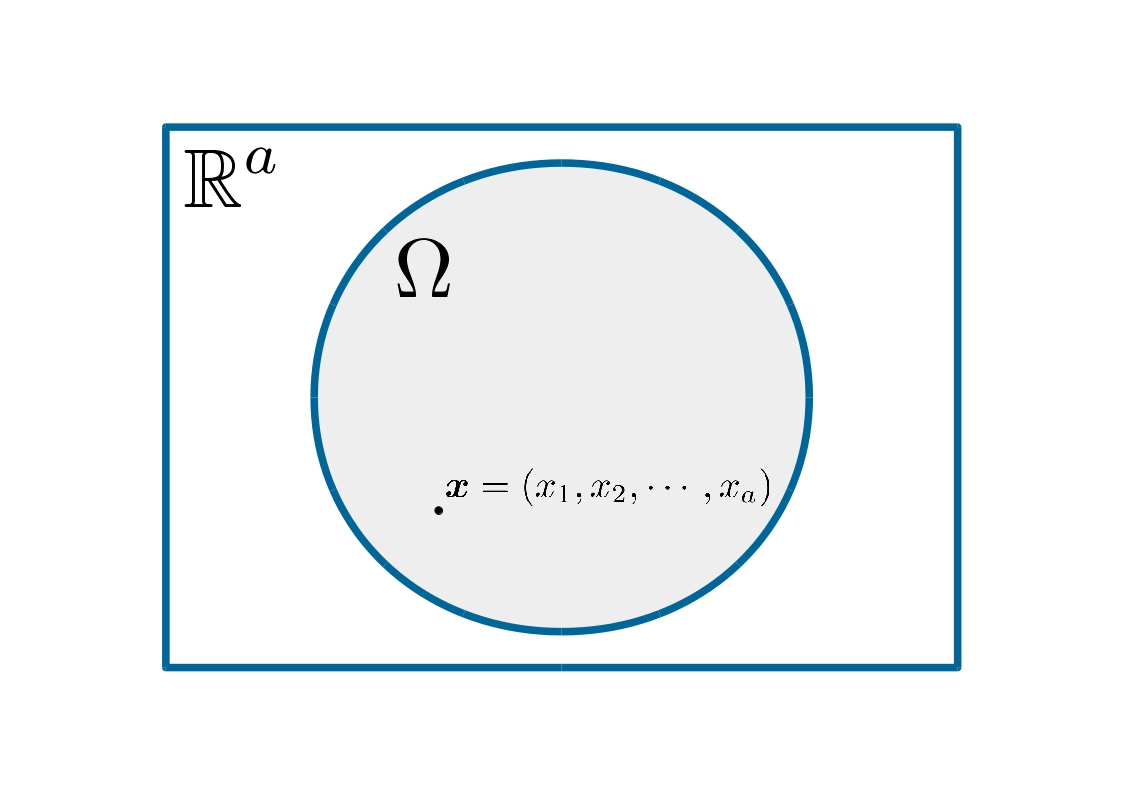
\includegraphics[width=10cm]{../img/ideaspace.jpg}
        \caption{$\mathbb{R}^{a}$上の空間$\Omega$と,その元である点$x$}
        \label{fig:f1}
    \end{center}
\end{figure}

また,この意見間の距離を定義すればこれらの点を元とする距離空間を定義することができる。距離の入れ方としてはユークリッド距離
\[d(x, y) = \sqrt{(x_{1} - y_{1})^{2} + \cdots + (x_{a} - y_{a})^{2}}\]
を考えることとする。

次に,「参加者」について考える。参加者は会議の中で自分の中にある意見を発言していくのであり,参加者それ自体は意見の集まりである。すなわち意見空間$\Omega$上の部分空間$X_{i}$が参加者$i$を表すとする。$x_{ik}$が人$i$のラベル$k$の意見であるとすると,人$i$が$s_{i}$個の意見を持っているとき,
\[X_{i} = \{x_{i0}, x_{i1}, \cdots , x_{is_{i}}\}.\]
一般に
\[X_{i}\cap X_{j} = \emptyset\ \ \  \text{when}\ \ \ i \neq j\]
である必然性はないが,このモデルでは上式を採用することとする。したがってモデルの中で扱う意見空間$\Omega_{0}$は,参加者が$N$人集まったとき,$X_{i}$の直和集合
\begin{align}\Omega_{0} &= \bigcup_{i = 1}^{N} X_{i} \nonumber \\
&= \sum_{i=1}^{N} X_{i} \end{align}
となる。

モデルの作成に際し,会議の進行に関していくつかの仮定をおいて考えていくことにする。これらの仮定が本質的であるような場合にはまた別のモデル化を考える必要があるが,ひとまず以下の仮定を受け入れることにして,その上でモデルを作成することにした。

仮定:
\begin{itemize}
    \item 一度に発言できる人は一人まで
    \item 一人当たりの発言時間は参加人数に依らない
\end{itemize}

このように仮定すると,会議という過程を,1つの時間発展するネットワークの生成過程であると見なすことができる。すなわちある参加者に必ず属する点をルールにしたがって各時刻ごとに選択していき,その時意見間の間にも与えられた別のルールによってエッジを結んでいくとする。このようにすると,終了時刻$K$が経過した時には,意見間のネットワークと,参加者間のネットワークを得ることができる。このネットワークの特性の中に,会議の質となりうる量があるとして,この描像のもとに意見$x$や参加者$X_{i}$の選択に関してのルールを与えていくことにする。

以降の議論では,特に必要のない限り,上で定めた記号と言葉を使い,「会議,意見,参加者」といった言葉は使わないことにする。

点$x$の選び方としては,
\begin{enumerate}
    \item 集合$X_{i}$を選び,その中から$x$を選ぶ方法
    \item 点$x$を選び,その点の情報から,$X_{i}$を決める方法
\end{enumerate}
の二つがある。

それぞれの場合について,$x$と$X$を選ぶ確率が互いに独立な場合と,そうでない場合にさらに分けて考えることができる。

したがって,考えるべきは
\begin{itemize}
    \item $X_{i}$の独立な選び方
    \item $x$の独立な選び方
    \item $X_{i}$が選ばれたときの$x$の選び方
    \item $x$が選ばれたときの$X_{i}$の選び方
\end{itemize}
の4つである。
